\begin{titlepage}

\newcommand{\HRule}{\rule{\linewidth}{0.5mm}} % Defines a new command for the horizontal lines, change thickness here

\center % Center everything on the page
%----------------------------------------------------------------------------------------
%	TITLE SECTION
%----------------------------------------------------------------------------------------
\HRule \\[0.4cm]
{ \huge \bfseries DROGEN}\\[0.4cm] % Title of your document
\HRule \\[1cm]
 %----------------------------------------------------------------------------------------
%	HEADING SECTIONS
%----------------------------------------------------------------------------------------


\Large Nikotin \\[1.5cm] % Major heading such as course name
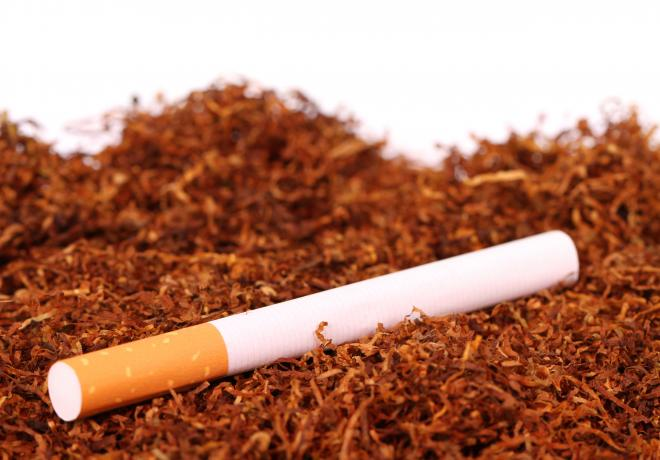
\includegraphics[trim = 0cm 0cm 0cm 0cm, clip=true, width= 12.5cm]{nikotin_titelgrafik} \\[1.5cm]
%----------------------------------------------------------------------------------------
%	AUTHOR SECTION
%----------------------------------------------------------------------------------------

\begin{minipage}{0.4\textwidth}
\begin{flushleft} \large
Lukas B�hler \& \\ J�r�me Landtwing % Your name
\end{flushleft}
\end{minipage}
~
\begin{minipage}{0.4\textwidth}
\begin{flushright} \large
Chemie 4. Jahr \\
Elsbeth Wyer% Supervisor's Name
\end{flushright}
\end{minipage}\\[2cm]

%----------------------------------------------------------------------------------------
%	DATE SECTION
%----------------------------------------------------------------------------------------
\large KSA Pf�ffikon\\ % Name of your university/college
\large Mai 2017\\[3cm] % Date, change the \today to a set date if you want to be precise


\vfill % Fill the rest of the page with whitespace

\end{titlepage}